\section{Fundamental group and monodromy action}
Fix a space $X$ and a vertex $x$ on it.

Recall that, a \emph{path} $\gamma$ in $X$ is a finite sequence of edges $e_1 e_2 e_3 \dots e_k$, where we allow inverses, such that $d_1 e_i = d_0 e_{i+1}$ for $1 \le i \le k-1$.
Denote $d_0 \gamma = d_0 e_1$ and $d_1 \gamma = d_1 e_k$.

We can concatenate two paths $\gamma_1$, $\gamma_2$ if $d_1 \gamma_1 = d_0 \gamma_2$ to get a path $\gamma_1 \cdot \gamma_2$ from $d_0 \gamma_1$ to $d_1 \gamma_2$.
For a vertex $x \in X$, we denote by $\mathbb{1}_x$ the path of length 0 starting at $x$, with the property that $d_0 \mathbb{1}_x = x = d_1 \mathbb{1}_x$ and $\gamma \cdot \mathbb{1}_x = \gamma$ and $ \mathbb{1}_x \cdot \gamma = \gamma$ whenever the concatenations make sense.

A \emph{loop} at $x$ is a path starting and ending at $x$. Concatenation defines a product on the set of loops.

The \emph{fundamental group} of $X$ at $x$ is essentially
\begin{equation*}
  \pi_1(X,x) = \langle \mbox{ loops } | \mbox{ faces }\rangle
\end{equation*}
There are multiple ways to make this definition precise. We will do this recursively.

We add \emph{generators} using edges.
\begin{enumerate}
  \item Start with just the vertex $x$.
  \item Add edges successive (while keeping the space connected).
  \item Every time the newly added edge $e$ forms a loop $\gamma$, add $\gamma$ as a generator to $\pi(X,x)$.
\end{enumerate}

We add \emph{relations} using faces.
\begin{enumerate}
  \item Add the faces one at a time.
  \item For each face, let $\gamma'$ be the boundary of the face starting at $y$.
  \item Add the relation $\gamma \cdot \gamma' \cdot \gamma^{-1}$ to $\pi_1(X,x)$ where $\gamma$ is a path connecting $x$ to $y$.
\end{enumerate}

\begin{remark}
  If you think that this definition is artificial and contrived, then you are correct. There is a very natural object called the \emph{fundamental groupoid} associated to the space $X$ which does not depend on the basepoint $x$.
\end{remark}


  \begin{ex}
    The fundamental group of $S^1$ has a single generator and there are no relations.
    Hence,
    \begin{align*}
      \pi_1(S^1) = \langle a \rangle \cong \bbz
    \end{align*}
    \begin{figure}[H]
    \centering
      % \includegraphics[width=0.5\textwidth]{example-image}
      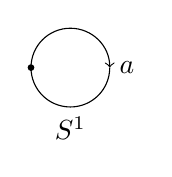
\begin{tikzpicture}[scale=0.5]
        \filldraw (0,0) circle (2pt);
\draw [->] (0,0) to [bend left=45] (1,1)  to [bend left=45] (2,0) node [right] {$a$};
\draw (2,0) to [bend left=45] (1,-1)  node [below] {$S^1$} to [bend left=45] (0,0);

      \end{tikzpicture}
      \caption{Fundamental group of a circle is $\bbz$.}
    \end{figure}
  \end{ex}

  \begin{ex}
    The fundamental group of $S^1 \vee S^1$ has a single generator and there are no relations.
    Hence,
    \begin{align*}
      \pi_1(S^1 \vee S^1) = \langle a, b \rangle \cong F_2
    \end{align*}
    which is the free group on two generators.
    \begin{figure}[H]
    \centering
      % \includegraphics[width=0.5\textwidth]{example-image}
      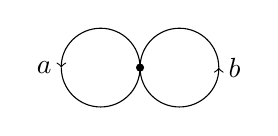
\begin{tikzpicture}[scale=0.5]
        \filldraw (0,0) circle (2.5pt);

\draw [->] (0,0) to [bend right=45] (-1,1) to [bend right=45] (-2,0) node [left] {$a$} ;
\draw (-2,0) to [bend right=45] (-1,-1) to [bend right=45] (0,0);

\draw [->] (0,0) to [bend right=45] (1,-1) to [bend right=45] (2,0) node [right] {$b$};
\draw (2,0) to [bend right=45] (1,1) to [bend right=45] (0,0);

      \end{tikzpicture}
      \caption{Fundamental group of $S^1 \vee S^1$ is $\bbz$.}
    \end{figure}
  \end{ex}

  \begin{ex}
    The fundamental group on cylinder is given by
    \begin{align*}
      \pi_1(\mbox{cylinder})
      &= \langle c, a b a^{-1} \mid  a b a^{-1} c\rangle \\
      &= \langle c \rangle \\
      &\cong \bbz
    \end{align*}
  \end{ex}

    \begin{ex}
      The fundamental group on torus is given by
      \begin{align*}
        \pi_1(\mbox{torus})
        &= \langle a, b \mid a b a^{-1} b^{-1} \rangle \\
        &\cong \bbz \times \bbz
      \end{align*}
    \end{ex}

  \begin{qbox}
    Find the fundamental groups of
    \begin{enumerate}
      \item $S^2$
      \item Mobius strip
      \item Klein bottle
      \item Real projective space
    \end{enumerate}
  \end{qbox}

  \begin{proposition}
    For any two vertices $x_1$, $x_2 \in X$ there exists an isomorphism
    \begin{equation*}
      \pi_1(X,x_1) \xrightarrow{\cong} \pi_1(X,x_2).
    \end{equation*}
  Henc, the fundamental group does not depend on the basepoint upto isomorphism.
\end{proposition}
  \begin{qbox}
    Pick a path $\gamma \in X$ from $x$ to $x'$.
    Conjugate by $\gamma$ to get an isomorphism between $\pi_1(X,x)$ and $\pi_1(X,x')$.
  \end{qbox}

\subsection{Monodromy}
\begin{proposition}
  A covering map $p:Y \rightarrow X$ induces a group homomorphism
  \begin{align*}
    p_* : \pi_1(Y,y) &\longrightarrow \pi_1(X,x), \\
    [\gamma] &\longmapsto [p(\gamma)].
  \end{align*}
  where $x = p(y)$.
  If $p$ is a non-trivial cover then $p_*$ is strictly injective i.e. $p_*\pi_1(Y,y)$ is a proper subgroup of $\pi_1(X,x)$.
\end{proposition}
\begin{proof}
  The group homomorphism is evident as $p$ preserves concatenation of paths.

  For injectivity, suppose $[p(\gamma)]$ is trivial inside $\pi_1(X,x)$.
  This means that $p(\gamma)$ is a product of terms of the form $\gamma \cdot \gamma' \cdot \gamma^{-1}$ where $\gamma'$ is the boundary of a face. Hence, $\gamma$ is a product of the lifts $\widetilde{\gamma} \cdot \widetilde{\gamma}' \cdot \widetilde{\gamma}^{-1}$.
  But $\widetilde{\gamma}'$ is also the boundary of a face as $p$ is a simplicial map.
  Hence, $[{\gamma}]$ is trivial $\implies$ $p_*$ is injective.

  $p_*$ is strictly injective as a path $y_1$ to $y_2$, both in the fiber over $x$, map down to a loop at $x$, say $\gamma$.
  By uniqueness of path lifting, there is no path that maps down to $\gamma$.
\end{proof}

\begin{theorem}
  Let $p:Y \rightarrow X$ be a Galois cover. Let $y$ be a vertex in $Y$ in the fiber over the vertex $x$ in $X$.
  Then there is a surjective group homomorphism
  \begin{align*}
    M:\pi_1(X,x) \longrightarrow \Gal(Y|X)
  \end{align*}
  whose kernel is $p_*(\pi_1(Y,y))$.
  We say that the loops in $X$ act via ``monodromy'' on the space $Y$.
\end{theorem}
\begin{proof}
  The map $M$ is defined as follows.
  Let $y$ be a point $y$ in the fiber over $x$ and let $\gamma$ be a loop in the base starting at $x$.
  Consider the unique lift $\widetilde{\gamma}$ starting at $y$.
  Because $p:Y \rightarrow X$ is Galois, there is a unique deck transformation $\varphi_{\gamma} \in \Gal(Y|X)$ sending $y$ to $d_1 \widetilde{\gamma}$.
  Then define
  \begin{equation*}
    M(\gamma) = \varphi_{\gamma}
  \end{equation*}
  In order to show that this map descends to $\pi_1(X,x)$ we need to show that $\gamma \cdot \gamma' \cdot \gamma^{-1}$ gets mapped to the trivial deck transformation, where $\gamma'$ is the boundary of a face.
  \begin{qbox}
    Check this.
  \end{qbox}

  The kernel of $M$ is the set of loops which lift to loops at $y$, which is the same as the set of loops in $X$ which are images of loops in $Y$, but this is precisely $p_*(\pi_1(Y,y))$.

  It remains to show that $M$ is a group homomorphism.
  Let $\gamma_1$ and $\gamma_2$ be two loops in $\pi_1(X,x)$. Suppose $d_1 \widetilde{\gamma_1} = y_1$ and $d_1 \widetilde{\gamma_2} = y_2$. Let $\varphi_1 = M \gamma_1$ and $\varphi_2 = M \gamma_2$ so that $ \varphi_1(y) = y_1$ and $\varphi_2(y) = y_2$.
  By unique path lifting it follows that the lift of $\widetilde{\gamma_1 \cdot \gamma}$ is the path that ends in $\varphi_1(y_2) = \varphi_1 \varphi_2 y$.
  Hence, $M$ sends $\gamma_1 \cdot \gamma_2$ to $\varphi_1 \cdot \varphi_2$.
\end{proof}


\begin{theorem}
  \label{theorem:fundamentalGroupQuotient}
  We can rewrite the above theorem as saying that if $p:Y \rightarrow X$ is a Galois cover with $p(y) = x$, then there is a short exact sequence of groups
  \begin{equation*}
    1 \rightarrow \pi_1(Y,y) \xrightarrow{p_*} \pi_1(X,x) \rightarrow \Gal(Y|X) \rightarrow 1
  \end{equation*}
\end{theorem}

\begin{qbox}
  Verify Theorem \ref{theorem:fundamentalGroupQuotient} for the coverings $(1)$, $(2)$, $(6)$, and $(11)$ of $S^1 \vee S^1$ in Figure \ref{fig:CoveringsOfS1S1}.
\end{qbox}

\begin{qbox}
  Verify Theorem \ref{theorem:fundamentalGroupQuotient} for the coverings
  \begin{align*}
    \mbox{Cylinder} &\longrightarrow \mbox{Mobius Strip} \\
    \mbox{Torus} &\longrightarrow \mbox{Klein Bottle} \\
    \mbox{Sphere } S^2 &\longrightarrow \mbox{Real projective space}
  \end{align*}
\end{qbox}







\begin{figure}[p]
\centering
  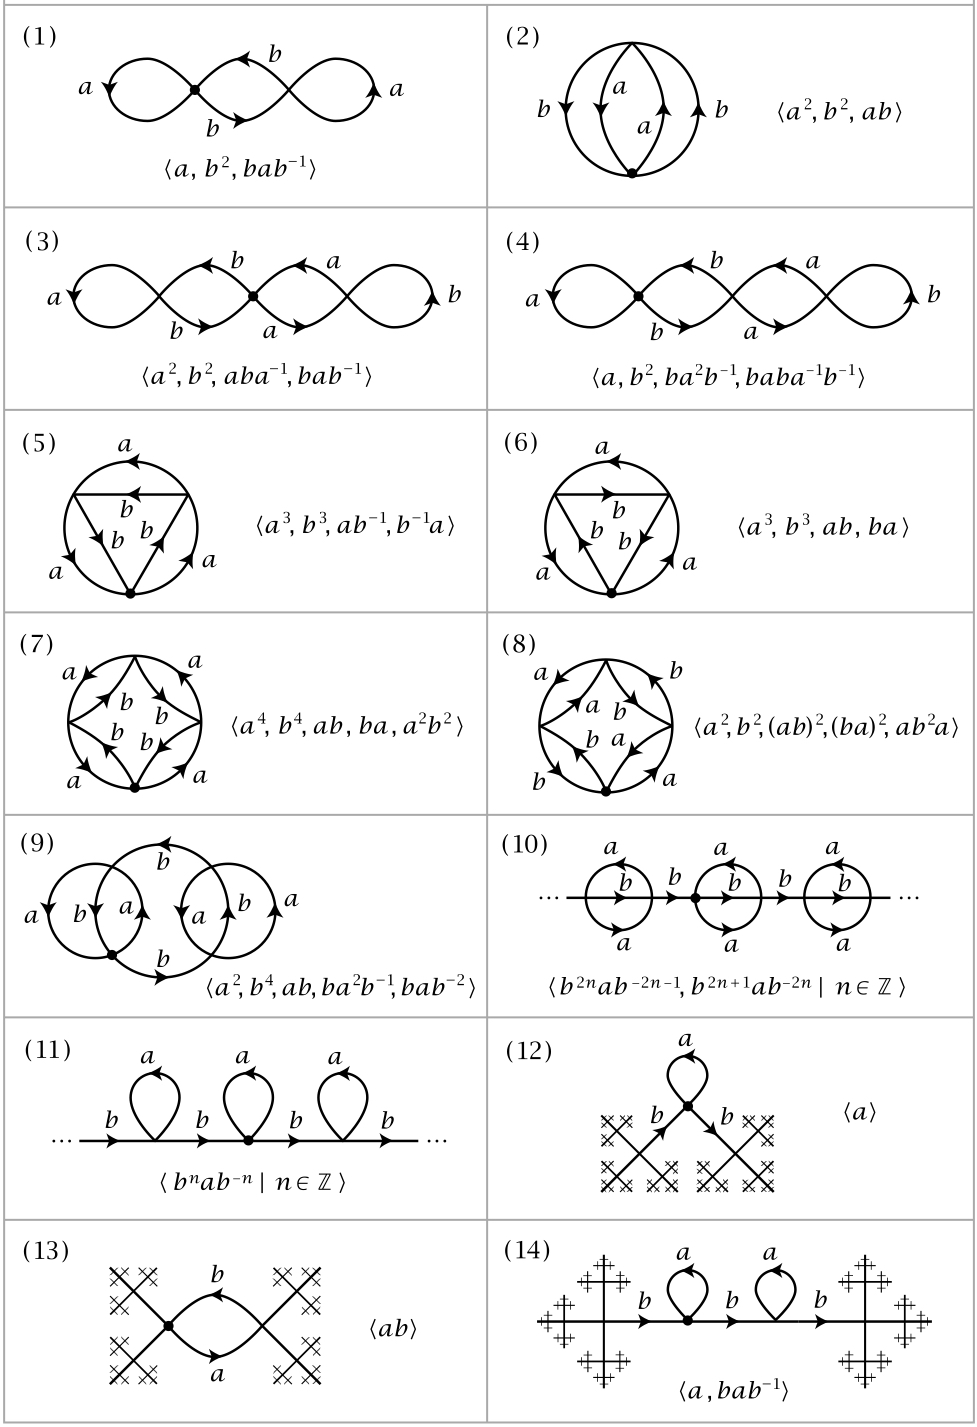
\includegraphics[width=\textwidth]{coveringsOfS1S1.jpg}
  \caption*{Coverings of $S^1 \vee S^1$. Image from Algebraic Topology, Allen Hatcher, Chapter 1.}
\end{figure}

\begin{figure}[p]
  \centering
  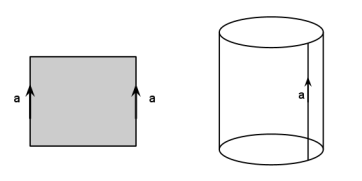
\includegraphics[width=0.65\textwidth]{cylinderGluingDiagram.png}
  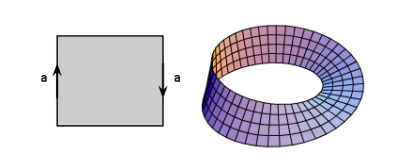
\includegraphics[width=0.65\textwidth]{MobiusStripGluingDiagram.png}

  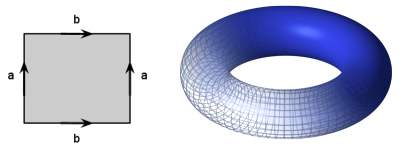
\includegraphics[width=0.65\textwidth]{torusGluingDiagram.png}
  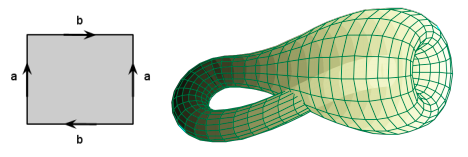
\includegraphics[width=0.65\textwidth]{KleinBottleGluingDiagram.png}

  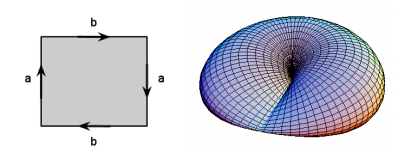
\includegraphics[width=0.65\textwidth]{RP2GluingDiagram.png}
  \caption*{Gluing diagrams for cylinder, Mobius strip, torus, Klein bottle, real projective space respectively. Images from BMC Notes on Surfaces by Maia Averett.}
\end{figure}
